\documentclass[12pt]{article}
\usepackage{amsmath}
\usepackage{amsfonts}
\usepackage[a4paper, margin=2.5cm]{geometry}
\usepackage{graphicx}
\usepackage{setspace}
\usepackage{parskip}
\usepackage{hyperref}
\usepackage{float}
\usepackage{booktabs}
\usepackage{glossaries}
\usepackage{subcaption} % in your preamble
\onehalfspacing
\usepackage[margin=2.5cm]{geometry}
\renewcommand{\baselinestretch}{1.5}
\usepackage{fontspec}
\setmainfont{Arial}
\usepackage{listings}
\lstset{
    basicstyle=\normalsize,
    breaklines=true,
    showstringspaces=false,
    numbers=left,
    numberstyle=\small,
    numbersep=8pt
}


\begin{document}











% Image optimization settings
% Configure image compression for XeTeX
\setkeys{Gin}{draft=false}

\setstretch{1.2}

\title{\Huge Autonomous Bitcoin Trading\\\vspace{1cm}\Large Documentation}
\author{
    \Large Gymnasium Thun\\
     26gs\\
    \vspace{1cm}
    \Large Submitted by:\\
    \vspace{0.5cm}
    \textbf{x}\\
    \vspace{2cm}
    \Large Supervised by:\\
    \vspace{0.5cm}
    \textbf{Dr. Geoffrey Ostrin}
}

% Title page
\pagenumbering{gobble}
\maketitle
\clearpage

% Abstract
\pagenumbering{roman}
\begin{abstract}
    This thesis examines the development of an autonomous Bitcoin trading algorithm, based on the observation that human emotion leads traders to act irrationally in the markets.
    The research combines technical analysis with algorithmic trading, employing a quantitative methodology that includes data collection, strategy development using Python, and testing strategies on historical price data. The implementation involves creating a custom backtesting framework, developing rule-based trading strategies, and deploying a live trading system on a Linux based server.

\end{abstract}
\clearpage

% Continue roman numbering from abstract
\section*{Foreword}
My interest in Bitcoin began in early 2022 after reading \textit{The Bitcoin Standard by Saifedean Ammous}. The book explores the history of money and argues that Bitcoin is a revolutionary form of hard money \footnote{A form of money that maintains its value over time, offering stability and reliability} superior to traditional currencies. The book sparked an interest in me, and I was drawn into the world of crypto. As a result, I spent more and more time watching charts and losing my mind over them. The idea of making profit from these seemingly random price movements fascinated me.
Trading profitably is straightforward: sell high and buy low. The practical implementation, however, is filled with uncertainty and  fight against your own instincts and emotions.
In addition to getting into crypto I also tried to learn to code since I wanted to make money on the side without having to leave my house. The first time I learned about automated trading algorithms I thought it was one of the hardest things to do. The combination of knowledge made me admire people who code in the finance space. It felt impossible but the more I tried the closer I got to something into the direction of a trading algorithm. With my matura thesis approaching I was pretty confident that I would be able to build an automated Bitcoin trading algorithm. 






I had no idea what I was getting myself into, and if I had known before, I would probably have never started. I spent more time than I intended and completely lost myself during the summer vacation. I totally forgot about the writing part and spent a lot of time just coding. This project grew much bigger than I initially thought, but I'm proud to present both the work outcome and the learnings I gained from it.





\clearpage

% Table of contents
\pagenumbering{roman}
\tableofcontents
\clearpage

% Start main content with arabic numbering
\pagenumbering{arabic}
\setcounter{page}{1}
\section{Introduction}
Making money in the capital markets is a complex activity that requires emotional control and discipline. Most individuals fail to make money on shorter time frames. Since computers do not suffer from psychological biases, automating the process offers the potential for more consistent decision-making. This thesis explores whether I can develop an autonomous trading algorithm that can generate me a consistent profit. 
This work does not aim to outperform professional trading firms, but rather to demonstrate the challenges of building a fully automated trading algorithm.
To that end my thesis will cover the entire development cycle of an algorithmic trading strategy. This will include finding a trading strategy, backtesting the trading strategy, applying the strategy to a live market, and evaluating the results.



The work is divided in three parts: Finding a strategy, Backtesting, and Live trading.

Finding a strategy can be done in multiple ways just by watching markets over longer time periods to get ideas, reading books about how other people were able to develop strategies and steal logic from them. In my case I will try to find a strategy by analysing the orderbook delta and identifying trends on the non-stationary \footnote{Non-stationary means not being still or fixed in one place; moving or changing rather than remaining constant.} bitcoin price. 

Backtesting is the process of testing a trading strategy on historical data to evaluate its performance. It is used to see if the strategy is worth automating.

Live trading is the process of executing a trading strategy on a live market. Here I will see if my strategy works in the real market and how it will behave. The strategy will be automated in Python. A major difference is that I will use two different Python programs for the backtesting process and the live trading algorithm.  


The project requires know-how in three key areas: Statistics, Programming and understanding how the cryptocurrency market operates. I need to apply statistical rules to check if my idea is worthless or has potential to make me a profit if I automate the execution process. Programming is just needed to make the process of testing or applying my ideas easy on large datasets since I have to test on time series. The algorithm will be written in Python and will run 24 hours a day seven days a week.





By the end of the project, I aim to deliver the following components:

\begin{itemize}
    \item Backtest results
    \item Trading strategy
    \item Trading algorithm program
    \item Live execution results
\end{itemize}




\newpage

\section{Theoretical Background}
Automating a trading strategy comes with many different challenges which are not obvious at first. In this section I will explain the basics needed to understand the trading market, algorithmic trading and challenges of creating a trading algorithm.







\subsection{What is trading?}
Trading means buying and selling financial assets like stocks, cryptocurrencies, or commodities, usually with the goal of making a profit. Traders try to buy at a low price and sell at a higher one, or profit from falling prices by selling high and buying back lower. Prices in financial markets change constantly, which creates opportunities and risks. There are many different types of trading, depending on the chosen timeframe, strategy, and how trades are managed. Losing is part of every strategy the goal is to lose less money than you win.
As trading is often seen as an easy way to make money it is important to understand that it is not easy. It is a skill that requires a lot of time and effort to master. Type of trading strategy does not matter there is no easy or fast way to success in trading. 

\subsubsection*{Algorithmic Trading}
In this thesis I will try to find success in the algorithmic trading niche, also know as Algo-trading or automated trading. This is a type of trading which uses computer programs to execute trades in financial markets based on predefined rules or mathematical models.  Inside of algorithmic trading there are again many different types. Some examples are: statistical arbitrage, trend following, and High-Frequency Trading. In terms of logic all these are not related at all and strategies are often very complex in these areas. 

My strategy is best described as a statistical signal-based strategy. As I try to find a metric that shows statistical evidence on which I can capitalized on. In financial markets we can profit by betting on a volatility change \footnote{a measure of how much and how quickly the price of a trading instrument fluctuates over time} or directional bias. Capitalizing from directional bias is as simple as buying if your directional bias positive and selling if we have a negative directional bias. (I am referring to positive and negative returns)



















\newpage
\subsection{What is Bitcoin?}

As my algorithm is trades the Bitcoin/USD pair, I want to explain what Bitcoin is.

Before explaining what Bitcoin is, it is important to first understand the fundamental problems of fiat money. 
The central issue lies in the centralization: governments and central banks hold complete control over the money supply. This control enables them to print money at will, there by increasing the supply and often causing inflation. As a result, the purchasing power of money decreases, which devalues people’s savings. In addition, monetary policy \footnote{actions undertaken by a nation's central bank to manage the money supply and credit conditions to achieve macroeconomic goals} 
decisions are frequently influenced by political considerations rather than sound economic principles, leading to poor economic outcomes. Ultimately, the system depends entirely on trust in governments to manage the money supply responsibly.


In 2009 a group or individual known as Satoshi Nakamoto published the White Paper of Bitcoin. The paper outlines the concept of a decentralized digital currency that would not be controlled by any central authority. Bitcoin is decentralized, meaning that no single entity controls the network. The money supply is limited to 21 million Bitcoins. Anyone with internet access can use Bitcoin. Transactions are immutable and cannot be changed once confirmed. Bitcoin is borderless and can be sent anywhere in the world.

In the figure \ref{fig:bitcoin_chart} we can see the price of Bitcoin over the years. The Y-axis is logarithmic to better visualize the strong increase in price. The X-axis shows the days since 2010.
\begin{figure}
    \centering
    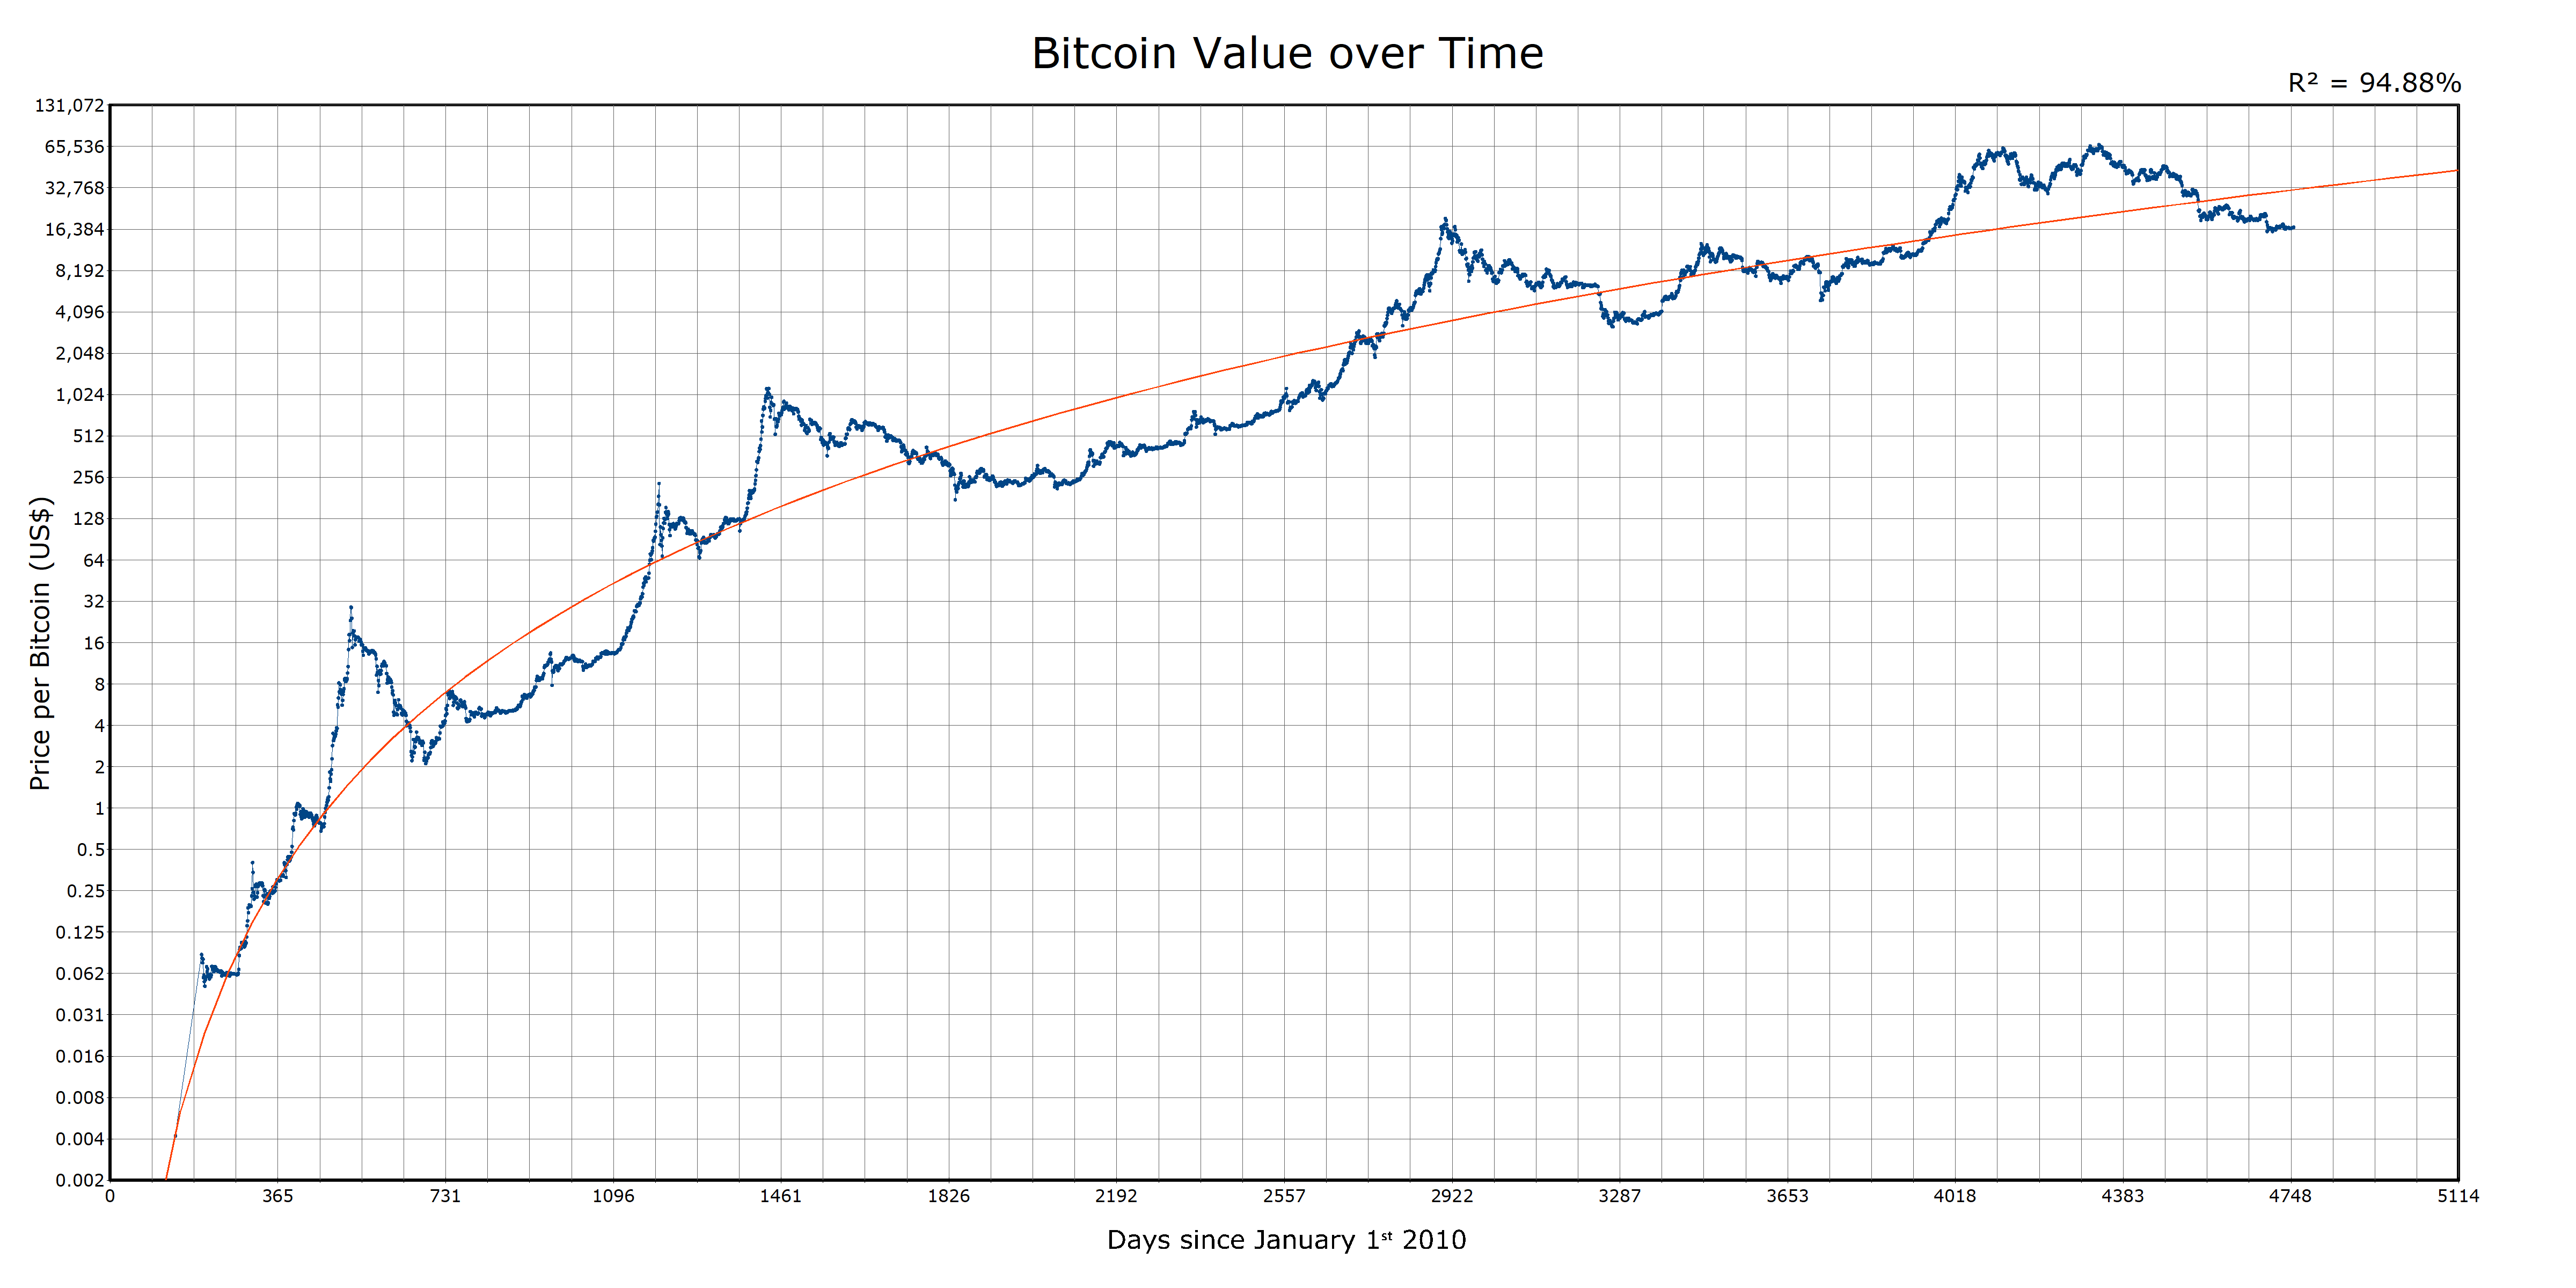
\includegraphics[width=0.9\textwidth]{imgs/bitcoin_price_over_years.png}
    \caption{Bitcoin price chart}
    \label{fig:bitcoin_chart}
\end{figure}



\newpage

\subsection*{Why trade Bitcoin?}
To prevent any misunderstanding, I want to clarify that I chose Bitcoin as an underlying asset for my trading strategy out of practicality and how my personal opinion about the asset is irrelevant. I read a few books explaining the reason for the creation of Bitcoin and the fundamentals behind it. I personally believe in the narrative of Bitcoin as a decentralized and inflation secure asset. However, this belief of mine plays no role in my trading algorithm. The goal of the trading algorithm is to react to signals which indicate market inefficiencies. These market inefficiencies can occur on any kind of asset in different magnitudes.
\subsubsection*{Data accessibility}
In the crypto market, real time and historical data is mostly free and accessible freely through public APIs. An API is a tool that allows programs to request and receive specific data from external services in this case, used to fetch real-time Bitcoin price and orderbook data from the coinbase crypto exchange. The data I based my strategy on is totaly free I just had to create my own timeseries in the traditional market I would have paid thousands of dollars for the same data.

\subsubsection*{Modern API infrastructure}
Some crypto exchanges offer modern API infrastructure which allow to automate trading. The exchange I chose Hyperliquid offers world class python implementation of their API. This allows me to carry out trades with a simple self written python script that implements their python sdk. \footnote{A python sdk is a software development kit for python. It is a collection of tools and libraries that allow developers to interact with a specific API.}



\subsubsection*{Entry barriers}
You can start trading crypto with as little as 10 USD no matter if the exchanges offers automated trading or just manual executed trades. While in the traditional market you need at least 10'000 USD to open an account for on a broker which offers automated strategy access.



These features make Bitcoin an interesting asset, both from a technological and financial perspective.




\newpage
\subsection{Efficient markets}
Making consistent profits in financial markets is difficult. Prices move in ways that often seem unpredictable, and most traders both discretionary and systematic struggle to gain a lasting edge. \footnote{An edge is a consistent advantage over the market. It can be achieved through superior information, better analysis, or a unique trading approach.}One explanation for this is the Efficient market hypothesis (EMH) which suggest that asset prices already reflect all available information, leaving little room for profitable opportunities.






If the EMH were fully accurate in practice, then even the most advanced trading algorithms and best discretionary traders would not be able to consistently beat the market. \footnote{Beating the market means achieving a higher ROI ("Return on Investment") than a certain benchmark. A common benchmark is the S\&P 500, which is an index including the 500 largest companies listed on U.S. stock exchanges. The S\&P 500 has had an average yearly return of about 10.33\% since 1957} Yet markets are not perfectly efficient, being heavily influenced by emotion, fear, and herd behaviour. Traders often fail to act on clear signals simply because it is psychologically hard to buy on a red day or sell while everybody is full of euphoria.


To make things even better depending on where you trade market can change in efficient. But still some of the most valuable assets like stocks, gold and Bitcoin prices are a reflection of human emotion pricing in information. Especially in the last few years with the introduction of spot Bitcoin ETFs a lot of volatility came in with big opportunities

Depending on the timeframe there are still a lot of inefficiencies from which individuals can make a profit from. I will try to act on short term inefficiencies with my trading algorithm because I only have about one month for the live test and it would not make sense to run an algorithm which holds a trade over weeks and takes a trade every two months. In addition my initial idea when I started of with my matura thesis was already based on short term signals.

It is possible to make a profit in the markets but it is not easy, not for everyone, and needs dedication. I am pretty sure I am able to make a profit. The question rather is if it is possible to do so in the limited time I have and at what scale.






\subsubsection*{Understanding Market Edge}
Before diving into strategy development, it's important to understand the concept of a market edge. An edge is a consistent advantage over the market that allows a trader to capitalize on market inefficiencies. Edge can have many different orgins some example are:
\begin{itemize}
    \item Superior information or analysis
    \item Faster execution or better technology
    \item Unique trading approaches that exploit market inefficiencies
    \item Better risk management techniques
\end{itemize}
Without a clear edge, even the most sophisticated trading system will struggle to generate consistent profits. The goal of systematic strategy development is to identify, validate, and exploit such edges in a repeatable way.








\subsection{Development of a Systematic Strategy}

\textbf{Idea Generation:}
The systematic strategy has to be based on a hypothesis that once signal X occurs the market is wrong and we can profit from the market correcting back to a fair value. This can be done by copying other strategies and applying them in a different way or in a different market. The approach I took was trying to make a discretionary strategy into a systematic one.



\textbf{Backtesting:}
After coming up with an idea we have to make a strict set of entry and exit conditions. We test the rules on historical data. This allows the developer to evaluate how the strategy would have performed in the past. This allows us to get a hint on how the strategy would perform in the future and if it is worth automating. 

\textbf{Optimization and Robustness Testing:}
After initial tests, parameters can be adjusted. A simple example would be adjusting the holding time of a trade.  Some inefficiencies can be corrected in minutes others might take a day or two it is up to us to find the right balance. Holding time is a simple example which doesn't bring a lot of risk with it if we test on different holding times. As long as we use a limited amount and have clear differences between the different holding times we can be sure that the strategy is robust. The biggest risk we face with backtesting is that we might overfit the strategy to the past data. An overfitted strategy looks great on historical data but will fail in the live market.

\textbf{Live Execution:}
If the backtesting results are promising and the strategy appears robust, it can be deployed live. Execution is handled by a algorithm running on a server, which listens to market data and acts as soon as the conditions are met. New things have to be taken in consideration here whicha are not a problem in backtests. One such thing is the time it takes to calculate the entry and exit conditions. This is a problem, as the price might change between when the actual entry conditions occur and when the entry signal is calculated.

Throughout this process, the focus remains on consistency and measurable results. Unlike human decision-making, a systematic strategy must behave identically entry and exit conditions. This makes it possible to evaluate, improve and automate trading in a transparent way.











\newpage
\section{Methodology}

\subsection{Project Overview}
The aim of this project was to design, test, and deploy a fully automated trading strategy for Bitcoin.
My development process consisted of four main stages. First, historical price data was collected to backtest strategies on.
In the second stage I try to develop an edge by analyzing the data I collected and define a signal from it.
In the third step, the entry and exit conditions are backtested on several months of historical data using a custom Python-written framework. Finally, if the results met predefined criteria (e.g. acceptable drawdown and stable returns), the strategy was deployed live on a PaaS that connects to the exchanges where the trades are executed in real time.

\subsection{Data collection}

% write about how this has to do with the EMH and why this offer new found edge 


I chose to create my own dataset because it offers a key advantage: it allows me to experiment with ideas and patterns that are less likely to have been explored before as I am not limited to the data provided by a platform. 
This increases the chance of discovering something new that might be missed when using more commonly available datasets.

There are platforms that offer orderbook delta data for free, but only for discretionary trading (i.e. they only display the data in a chart and do not provide it as a downloadable time series). My idea was to create a Python script which hits the API in one-minute intervals and stores the data inside a Postgres database. I have been hosting the data mining script on my PaaS since March 11, 2025 \href{https://customchart-production.up.railway.app/#}{Live database connection}.

The creation of the time series was done through a public exchange API\footnote{API stands for Application Programming Interface. It is a tool that allows programs to request and receive specific data from external services—in this case, used to fetch real-time Bitcoin price and orderbook data from the Coinbase crypto exchange.}, with data fetched in one-minute intervals and stored inside a database on a PaaS\footnote{PaaS stands for Platform as a Service. It is a cloud computing model which gives developers a platform to host their applications so that they are globally accessible on the internet and run 24/7}.


In my dataset, I calculate the 1\%, 2.5\%, and 5\% delta of the orderbook. Additionally, I include the current Bitcoin price and the corresponding timestamp. The program I wrote collects data by sending API requests to the Coinbase Exchange API at one minute intervals. It retrieves both the current Bitcoin price and a full snapshot of the orderbook at that moment. A complete snapshot is necessary to calculate orderbook deltas at different percentage depths accurately.


\newpage
\begin{equation}
    \Delta_{OB} = \sum_{i=1}^{n} V_{bid_i} - \sum_{i=1}^{n} V_{ask_i}
    \label{eq:orderbook_delta}
\end{equation}

I got the formular for the orderbook delta calculation from: \href{https://academy.hyblockcapital.com/indicators/orderbook/bids-and-asks-delta?utm_source=chatgpt.com}{Hypeblock capital}

% The main problem I faced here is that price time series in trading are usually constructed so that each data point represents the closing price of a fixed time interval (e.g. every minute at \texttt{xx:00}). If data points are missing or misaligned (e.g. recorded at \texttt{xx:00:15} instead of \texttt{xx:00:00}), then the time series becomes irregular and any backtest conducted on it would be flawed.
% A few key things flow together here which make it difficult to get a perfectly aligned timeseries. As python runs in a single threaded \footnote[3]{A python program runs by executing line after line.  Using the thread} 






\subsection{Framework}
Now before diving into the development of a systematic trading strategy I want to explain what kind of services we need and how we can use them to our advantage.

\subsubsection*{Broker}
In order to buy and sell Bitcoin we need an exchange to trade on and the exchange should offer a modern API infrastructure, which allows my trading algorithm to send commands to the exchange to sell and buy Bitcoin. The most fitting exchange for this is Hyperliquid. As it offers a modern API infrastructure and a very comprehensive documentation with a lot of examples \href{https://github.com/hyperliquid-dex/hyperliquid-python-sdk}{Hyperliquid Python SDK}.   

\subsubsection*{Hosting services}
Running the algorithm on my personal computer is not an option as it would require me to have my computer running 24/7. This is not feasible and would also require me to have a stable internet connection. For this reason I need a hosting service that can run my algorithm 24/7. I chose Railway since it is very simple to use and I already know how to host my code there as I have been using it for a long time for other projects. Railway is a PaaS (Platform as a Service) which allows me to host my code on a server and run it remotely.

\subsubsection*{Backtesting Python libary}
A python library is a collection of tools and libraries that allow developers to interact with a specific API. For backtesting I chose Vectorbt as it offers a comprehensive set of tools for backtesting and has a very comprehensive documentation with a lot of examples \href{https://github.com/polakowo/vectorbt}{Vectorbt Documentation}.








\newpage
\subsection{Defining goals}


The most difficult part of developing a trading algorithm is finding a strategy that is actually worth integrating. As explained in the Efficient Markets section, it is in principle possible to find a strategy that generates profit. The problem is that finding a strategy which consistently makes money and outperforms the market is still extremely difficult.

Before I start searching, I need to define what I am searching for. To do this, I use the S.M.A.R.T. goal framework (Specific, Measurable, Attainable, Relevant, and Time-bound), as described in the book \href{https://www.amazon.com/Building-Winning-Algorithmic-Trading-Systems/dp/1118778987}{\textit{Building Winning Algorithmic Trading Systems}} by Kevin J. Davey.

\subsubsection*{Goals}

\begin{table}[h]
\caption{SMART Goals for Strategy Development}
\begin{tabular}{p{0.2\textwidth} p{0.35\textwidth} p{0.35\textwidth}}
\toprule
Criterion & Goal & Explanation \\
\midrule
Specific & Strategy trades Bitcoin/USD pair & Asset is clearly defined \\
\addlinespace
Measurable & Target Sharpe ratio between 1--2 \footnote{The Sharpe ratio is a measure of risk-adjusted return. It compares the average return of a strategy to its volatility. A higher Sharpe ratio indicates a better balance between risk and return. A Sharpe ratio between 1 and 2 is considered decent in most financial contexts.} & Performance can be compared objectively \\
\addlinespace
Attainable & Approx. 20 trades per month & Fits within time and data constraints \\
\addlinespace
Relevant & Focus on stability and consistency, not outperforming the market & Aligns with project objectives \\
\addlinespace
Time-bound & Two months to find and test a strategy & Aligns with thesis timeframe \\
\bottomrule
\end{tabular}
\end{table}



%Starting of with searching for a potential strategy I already had a few ideas coming from discretionary trading approaches where I saw a potential to implement as a systemmatic set of rules. Just by reading tweets, watching crypto charts, and by playing with platforms offering various kinds of indicators. %One of the most significant advantages of crypto markets is the accessibility and granularity of trading data. Most major exchanges offer free public APIs that provide real-time and historical price data, often down to the minute or even second. This includes not only price and volume, but also open interest, funding rates, and even aggregated orderbook data in some cases. In contrast, similar datasets for traditional assets (e.g., stocks or futures) are often locked behind expensive data vendors or limited in granularity. The open nature of crypto data allows independent developers and researchers to prototype, test, and iterate much more rapidly — making it an ideal environment for building and evaluating automated strategies.


% Smart strategy explination  why a goal is neede
% from where did I take inspiration
% book I read
% testing testing and more testing
% where could I have done better
% how do the results macht with the live test
% Premutation tests and strategy development








\newpage
\subsection{Robustness Check via Resampled Strategy Variants}

Instead of running a single backtest of one strategy, we generate $M$ variations of the same base entry condition. Each variation trades a different random subset of the original trade signals and use different holding periods. It is important to note that we could use a different parameter than the holding periods but for my strategy it made moste sense. Changing other parameters would have introcuced the risk of overfitting our strategy to our historical data.

Formally, let the base entry condition identify $N$ candidate trades. For each variation $v \in \{1,\dots,M\}$ we sample a fraction $p_v \in (0,1]$ of these $N$ signals (without replacement) and assign a holding period $H_v$. The net performance of each variation is then computed after applying transaction costs $c$ that include both fees and slippage.

The key insight is that if the entry condition contains no edge, the distribution of net returns across the $M$ variations will concentrate around zero or negative values once costs are applied. In contrast, if a genuine edge is present, the majority of variations will show consistently positive outcomes even though each trades a different subset of signals. We gain a better insight into our strategy signals by comparing the difference in performance between different fraction sizes. I will explain why this is important once I explain my strategy logic.

One might ask why not simply reverse the signal. Let $\bar{r}$ denote the average gross return per trade of the original signal. A reversed signal would only be profitable if $|\bar{r}| > c$ and $\mathrm{sign}(\bar{r}) < 0$ often enough. In practice this condition rarely holds, since most weak or noisy signals satisfy $|\bar{r}| \leq c$, making reversal unprofitable after costs.


\subsubsection*{Walk-forward testing}
Even if we search for a strategy by using this multi parameter testing framework. In order to prevent to being lucky with a good looking parameter combination I run the same strategy on new data. This way I can see if the strategy is still profitable and if it is I can be sure that it is not just a lucky hit.
First test is done on 40'000 minutes of data if the strategy is profitable I run it on 60'000 minutes of data. If the strategy is still profitable I run it on 200'000 minutes of data. 95\% of the time the strategy goes from a good looking strategy to a bad one.








\newpage







\begin{figure}[H]
    \centering
    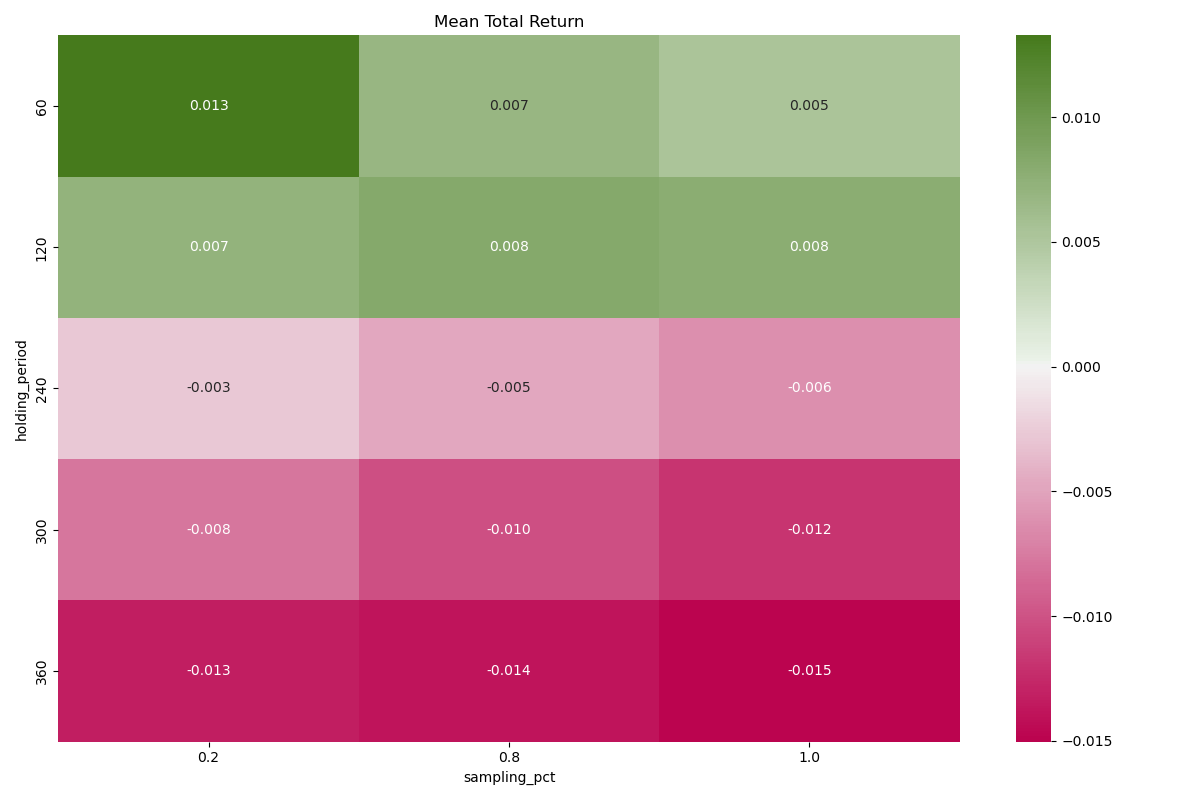
\includegraphics[width=\textwidth,height=0.7\textheight,keepaspectratio]{imgs/showcase_market_simulation.png}
    \label{fig:bullish_outliers_comparison}
    \caption{Backtest average return comparison}
\end{figure}

In the heatmap above you can see the results for a simple strategy backtest on a 40'000 minutes timeseries. Strategy logic does not matter yet. The x-axis shows the sample size and the y-axis shows the average return over the different test runs.
A value is colored green if the average return is positive and red if it is negative. The stronger the color the higher or lower the average return is.


I realeased a compensatied version of this Backtesting framework on my github page. It is called \href{https://github.com/AJslashTracey/signal_search_strategy}{signal\_search\_strategy}. 
The testing and analysis methodology presented here mirrors what I use in my actual trading operations. While my original codebase contains complex trading signals and closely interlinked components, I have developed a simplified version to carrying the same logic and concepts. This implementation maintains all essential components of the system, including signal processing, cost calculations, and performance measurements, while removing private and project-specific elements. I created this streamlined version to ensure others can both verify the methodology and run the system themselves, without getting overwhelmed by technical complexities or encountering private trading information. \footnote{The public repository is optimised for integration with other projects.}











\newpage
\subsection{Strategy example}
For showcasing purposes I will run a backtest on a strategy which is based on two different moving averages. We buy once the short moving average crosses the long moving average from below and sell once the short moving average crosses the long moving average from above.


\subsubsection*{Python implementation}
\begin{lstlisting}[language=Python]
import vectorBT as vbt
fast_ma = vbt.MA.run(price, 10)
slow_ma = vbt.MA.run(price, 50)
entries = fast_ma.ma_crossed_above(slow_ma)
exits = fast_ma.ma_crossed_below(slow_ma)
\end{lstlisting}

\begin{figure}[h]
    \centering
    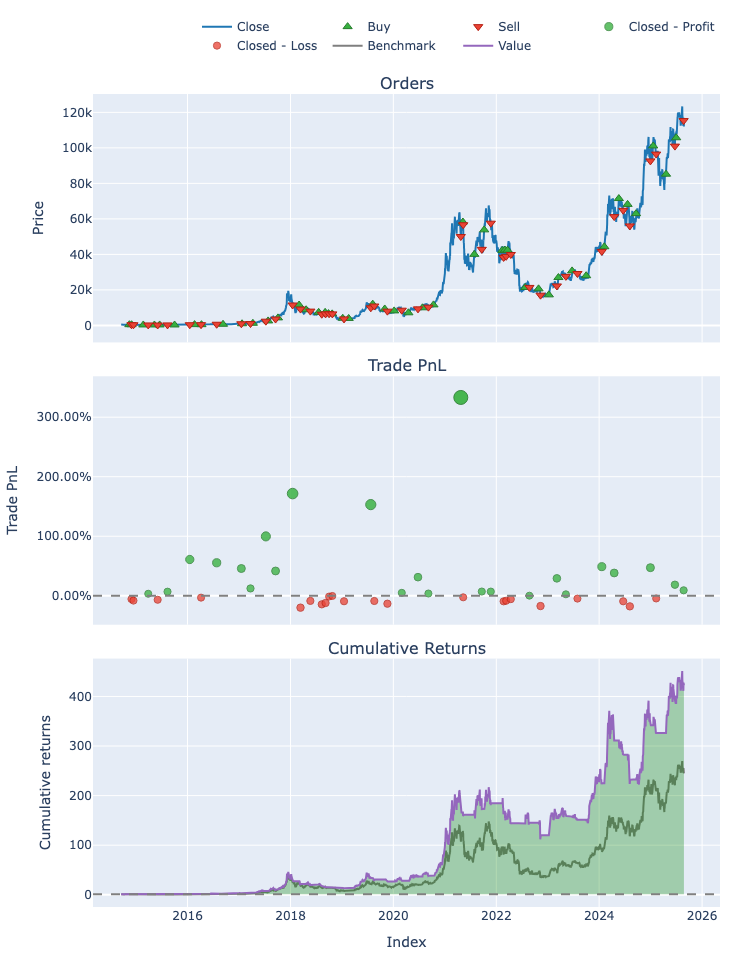
\includegraphics[width=0.7\textwidth]{imgs/strat_show_case_btc.png}
    \caption{MA cross strategy}
    \label{fig:ma_cross_strategy}
\end{figure}

\newpage

\subsection{Final strategy}
The area where I saw the most potential was the orderbook delta (see Equation \ref{eq:orderbook_delta}). My hypothesis was that, since it directly reflects the relationship between buyers and sellers at specific price levels, it could serve as the basis for a statistical signal. By running volatility and directional bias tests under various orderbook delta conditions, I aimed to identify patterns that might be predictive of short-term price movements.




\begin{figure}[h]
    \centering
    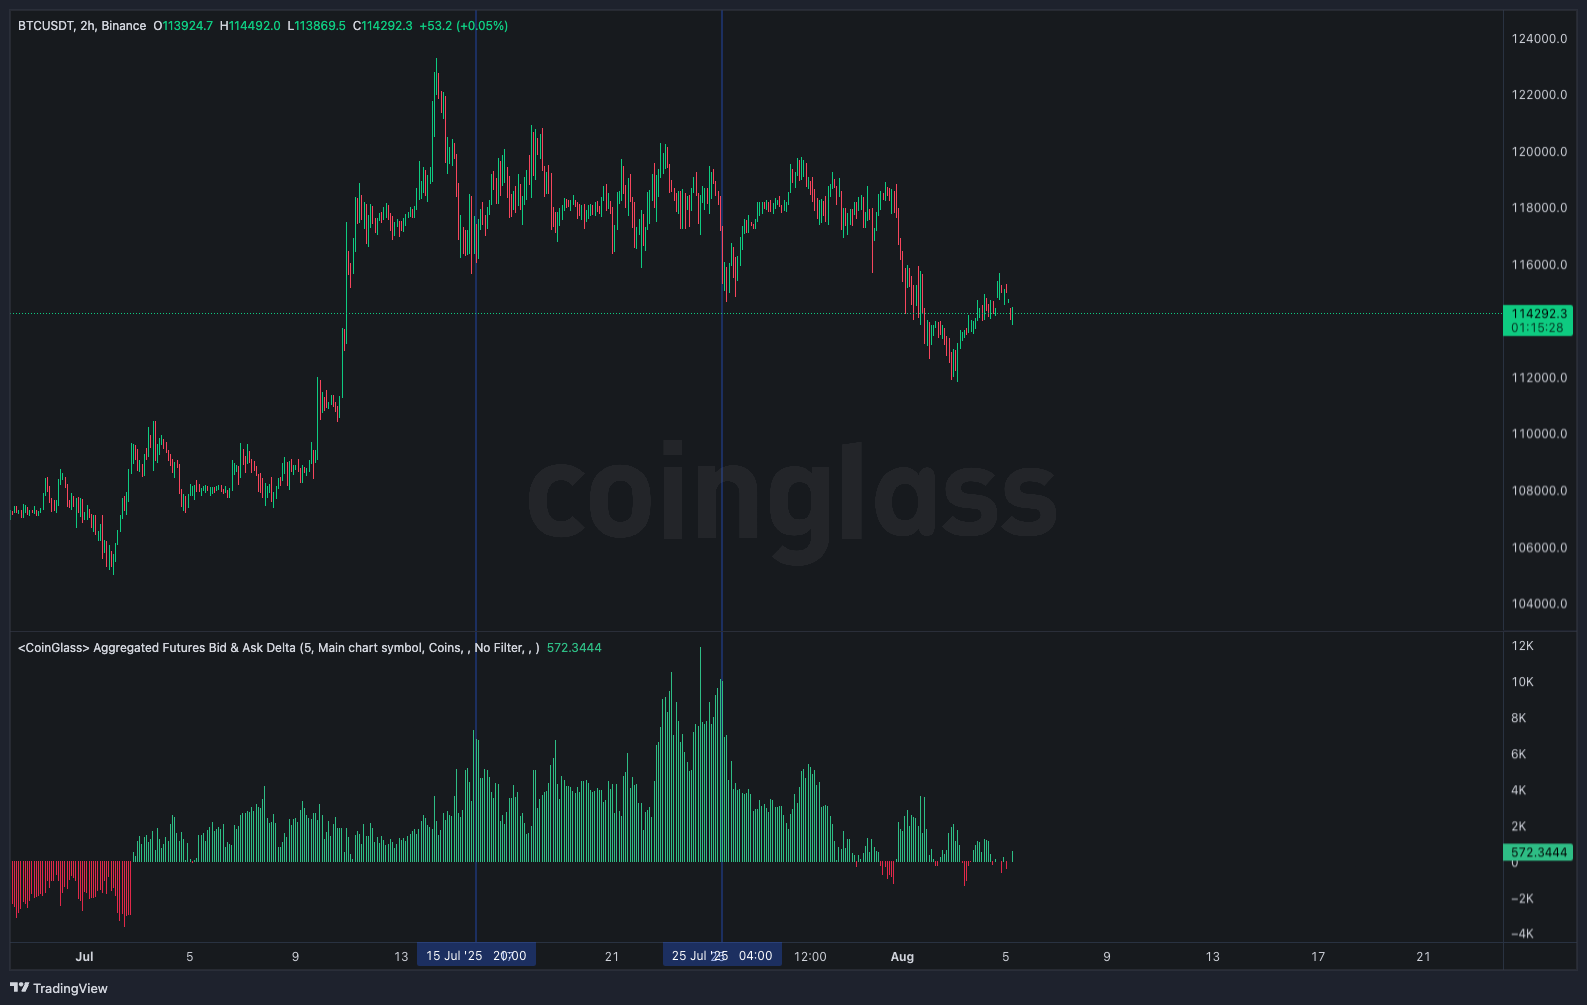
\includegraphics[width=0.9\textwidth]{imgs/showcase_chart.png}
    \caption{orderbook delta visualization showing price action (top) and corresponding delta values (bottom)}
    \label{fig:orderbook_delta}
\end{figure}




As shown in Figure \ref{fig:orderbook_delta}, the orderbook delta provides valuable insights at extreme values. The chart displays two key components:
\begin{itemize}
    \item The price action (top chart) shows the actual Bitcoin price movements
    \item The orderbook delta (bottom chart) represents the imbalance between buy and sell orders
\end{itemize}

A high orderbook delta value indicates substantial buy orders below the current price. This creates a strong support level, as sellers would need significant pressure to break through these orders. Even if sellers manage to push through, these accumulated buy orders often create buying pressure that can lead to price support or potential rebounds.
















\newpage
\subsection*{Strategy backtest implementation}


\subsubsection*{Sharp ratio}
To compare different strategies we should not ourselvs to only compare the total return a strategy achieves. Especially when we are not trying to outperform the market. Investing is associated with risk a good comparison between different strategies is to compare how much return we get for the risk we take.
The sharpe ratio does exactly this. It is a measure of the return per unit of risk. I used this as the main metric to compare strategies. Following formular is used to calulate the sharpe ratio:


\begin{equation}
    \text{Sharpe ratio} = \frac{\text{Average return $t$}}{\text{Standard deviation $t$} \footnote{$t$ is the time span over which we calculate the average return and the standard deviation} }\cdot \sqrt{98280} \footnote{98280 is used to annualize the Sharpe ratio we do this in order to compare the Sharpe ratio with the Sharpe ratio of other strategies or funds}
\end{equation}

There are different variations of the sharpe ratio. The orginal version as defined by WIlliam Sharpe, uses the return of a strategy compared to a risk free rate, divided by the standard deviation of the return.
How ever in the crypto industry the is no universally accepted risk free rate. 

\begin{equation}
    \text{Sharpe ratio} = \frac{\text{Average return $t$ - Risk free rate}}{\text{Standard deviation $t$}  }
\end{equation}

\subsubsection*{Backtesting results}

\begin{itemize}
    \item average sharpe ratio $1.55$ \footnote{The $\overline{SR}$ is the average Sharpe ratio over different walkforward periods}
    \item Over a time period of 137 days a return of $2.7\%$ was achieved
\end{itemize}


\subsubsection*{Backtest parameters}

\begin{itemize}
    \item A stop lost of $2\%$
    \item Exit is 120 minutes after entry or if a regime change occurs
    \item fees of $0.0003\%$ and slippage of $0.0001\%$
    \item accumulate $=$ True \footnote{This allows us to open multiple trades at the same timei}
\end{itemize}

\newpage
\subsubsection*{Code entry conditions}

\begin{lstlisting}[language=Python]
    # Entry conditions
    entries = (df['context'] == 'b') & (df['trend'] == 'Uptrend')
    
    
    # Exit after 120 minutes
    time_exit = exitSlots.shift(120).fillna(False)
    
    # Exit on trend change
    trendChange = (df['trend'] != df['trend'].shift(1))
    
    #Or statment to exit
    exits = trendChange | time_exit
    

\end{lstlisting}





\newpage
\subsubsection*{Entry conditions calculations}
I have to give more context about the entry conditions. \textbf{df\_temp} is just a variable to which I assign a timeseries dataframe \footnote{A dataframe is a two dimensional array with rows and columns} with different kind of metrics inside of it. The entry conditions are defined by two boolean conditions:


\subsubsection*{Outlier context}


\begin{lstlisting}[language=Python]
    df_temp['outlier_context'] == 'b'
    df_temp['trend'] == 'Uptrend'
\end{lstlisting}

As shown in Figure \ref{fig:outlier_context}, the dataframe contains various metrics that we use for our trading decisions:

\begin{figure}[h]
    \centering
    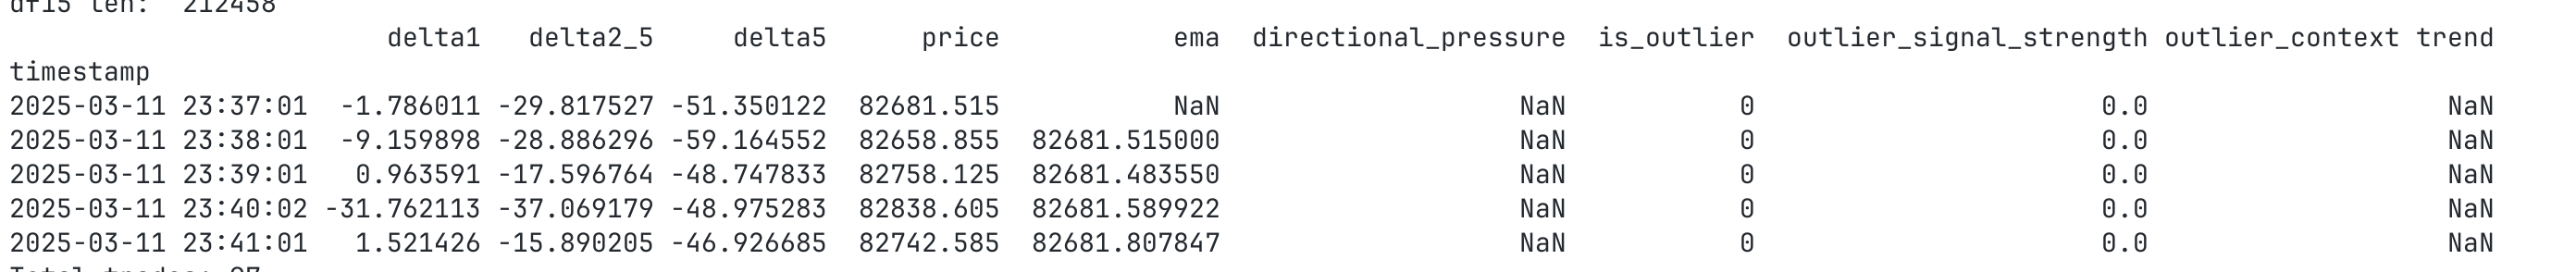
\includegraphics[width=0.95\textwidth]{imgs/dataframeHead.png}
    \caption{}
    \label{fig:outlier_context}
\end{figure}


The column $is\_outlier$ is a binary signal column if the current current orderbook delta value $\Delta_t$ is further than two standard deviations from the mean $\overline{\Delta}_{1440}$ of the orderbook delta.
$outlier\_context$ is a string column that has a value of \textbf{b} if $\Delta_t$ has a postive Z score and \textbf{s} if it has a negative Z score.

\subsubsection*{Market Structure and Trend Identification}

To identify trends in Bitcoin's price, we use a combination of price movement analysis and moving averages. The main challenge is to distinguish between real trends and temporary price movements. We start by converting our 1-minute price data into OHLC \footnote{OHLC stands for Open, High, Low, and Close. It is a type of data that is used to represent the price action of an asset over a period of time and is also known as a candlestick chart.} 240 minute data to better see the overall market direction.

\subsubsection*{Price Movement Analysis}
The core of our trend analysis looks at how price moves over time. We use two main indicators:

1. The derivative (rate of change) of a moving average:
\begin{equation*}
    \frac{d}{dt}\text{MA} = \text{Current MA value} - \text{Previous MA value}
\end{equation*}
When this derivative is positive, it indicates an upward trend, and when negative, a downward trend.

2. Price levels comparison:
We compare current prices with previous highs and lows using a window of time ($w$). This helps us confirm if we're really in a trend:
\begin{equation*}
\text{Trend}_t = \begin{cases}
    \text{Uptrend} & \text{if price is making higher highs} \\
    \text{Downtrend} & \text{if price is making lower lows} \\
    \text{Ranging} & \text{otherwise}
\end{cases}
\end{equation*}

\subsubsection*{Support and Resistance}
We also look at support and resistance levels to strengthen our trend analysis:

\begin{itemize}
    \item Resistance: Price levels where buying pressure tends to stop price from falling further
    \item Support: Price levels where selling pressure tends to stop price from rising further
\end{itemize}

The slopes of these levels help us determine trend strength. For example, rising support and resistance levels indicate a strong uptrend, while falling levels suggest a downtrend.

\subsubsection*{Final Trend Determination}
To make the final decision about the trend, we combine all these factors:
\begin{equation*}
\text{Final Trend} = \begin{cases}
    \text{Uptrend} & \text{if } \frac{d}{dt}\text{MA} > 0 \text{ and making higher highs} \\
    \text{Downtrend} & \text{if } \frac{d}{dt}\text{MA} < 0 \text{ and making lower lows} \\
    \text{Previous Trend} & \text{if moving average confirms} \\
    \text{Ranging} & \text{if no clear direction}
\end{cases}
\end{equation*}

This approach helps us filter out market noise and identify real trading opportunities. We only take trades when all these factors align, which increases our chances of success.





\newpage
\section{Results}

The first version of my trading algorithm was started on the 20th of July 2025. On average there is one signal per week. So it took me a week to find out that my algorithm was not working correctly. The problem was that the signal calculation was not the same as in my backtest. My backtest codebase became so big that I mixed things up and implemented the wrong logic.
I was not able to find the problem and kept updating it till I got about similar results as in my backtest. I will later dive deeper into why it is such a complicated problem to implement the backtest logic into a live trading algorithm.
On 10th of August I was able to make the algorithm nearly match the entry signals of my backtest. I had to stop trying to make the algorithm work exactly as in my backtest as time was running out. 14h of August first few trades were taken. 
I initially started two algorithms but one was such a failure that I was forced to stop it.






\subsection{Backtest results}
So there are two different backtest results the I want to show here. The results I got before the trading algorithm was implemented. And the results I got after the trading algorithm was implemented.
The results I got before the implementation were the signals based on which I decided to chose this particular strategy.

\subsubsection*{Backtest results before implementation}


\begin{figure}[h]
    \centering
    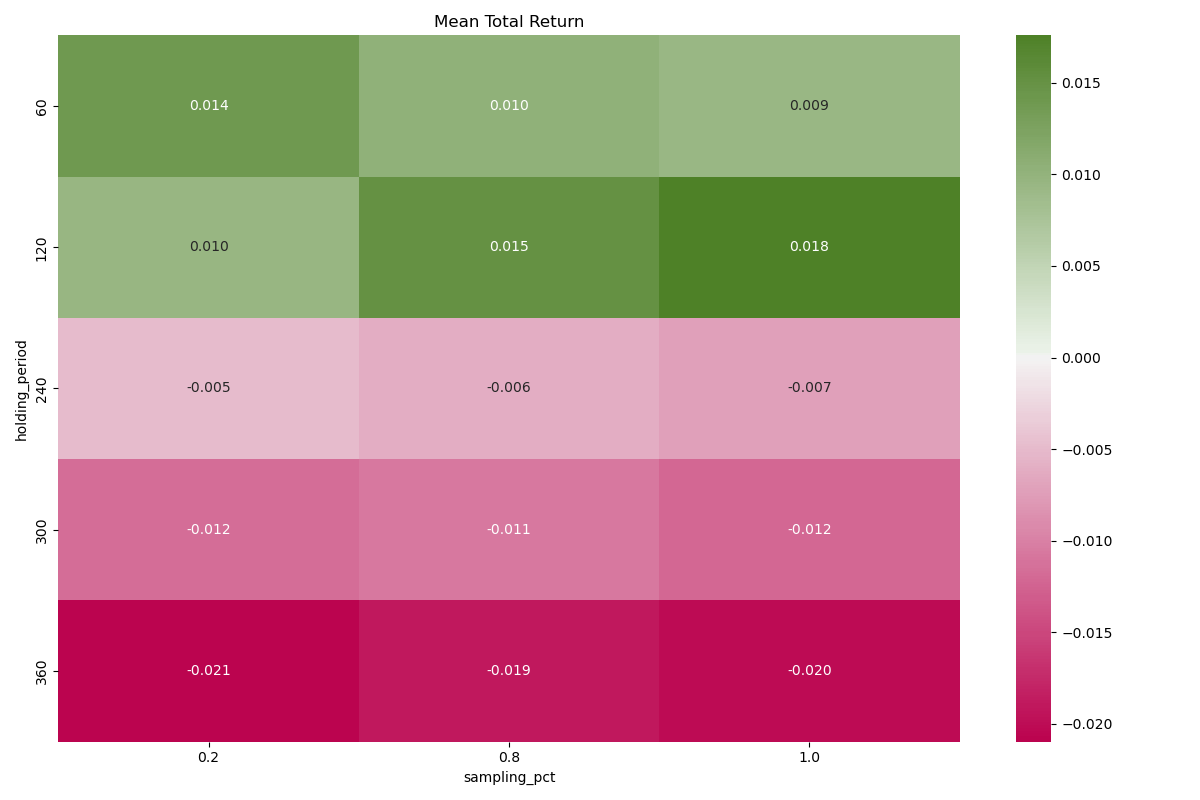
\includegraphics[width=0.9\textwidth]{imgs/backtest_results_ma.png}
    \caption{Backtest results before implementation}
    \label{fig:backtest_results_before_implementation}
\end{figure}

In the figure you can see the results of backtest I ran with different parameter settings. 
The results from the robustness ch  eck reveal important differences between holding periods. While both 60-minute and 120-minute horizons produced positive average returns, their behavior across sampling sizes diverged. At 60 minutes, average returns decreased as more trades were included, suggesting that profitability was driven by a smaller subset of favorable signals and may not generalize well. In contrast, the 120-minute horizon showed the opposite effect: returns increased with larger sampling sizes, indicating that the entry condition is more stable and benefits from scale. For holding periods of 240 minutes and longer, the strategy consistently generated negative results across all sample sizes. This confirms that the signal only provides an edge in the short term, and that profitability quickly decays if trades are held for too long. Taken together, these findings illustrate how robustness testing can uncover whether a strategy’s apparent profitability stems from a genuine, scalable edge (as in the 120-minute case) or from overfitting to a small number of lucky trades (as in the 60-minute case).

 



\subsection{Logic behind strategy}
 

\subsection{Trend identification}


\subsection{Extrem price identification}



\newpage


\newpage




\newpage
\section{Discussion}


\newpage
\section{Appendix}












\end{document}
